\chapter{Implementace aplikace}\label{chap:AppImplemetation}

Na předchozích stránkách teto práce byly popsány zásobníkové automaty, specifikace aplikace a technologie, které v této práci používám. Následující stránky se budou zabývat již samotnou implementací aplikace. Nejprve se zaměřím na to, jak vůbec reprezentovat zásobníkový automat v kódu. Následovat pak bude část zaměřující se na samotný simulátor a v poslední části se zaměřím na menu, tvorbu automatů pomocí formuláře, nahrávání souborů a jejich ukládání do paměti.

\section{Reprezentace zásobníkových automatů v kódu}

Abych mohl se zásobníkovými automaty pracovat v aplikaci, musel jsem mít způsob, jak je reprezentovat v kódu. Vytvořil jsem si tedy třídu PushdownAutomata, viz kód~\ref{src:PushdownAutomataDefinition}. Tato třída obsahuje jako atributy jednotlivé části definice zásobníkových automatů a dvě metody potřebné pro simulátor.

\begin{lstlisting}[label=src:PushdownAutomataDefinition, caption={Deklarce třídy PushdownAutomata}]
    class PushdownAutomata{
        states: State[];
        inputSymbols: InputSymbol[];
        stackSymbols: StackSymbol[];
        initialState: State;
        initialStackSymbol: StackSymbol;
        acceptingState: State[] | null;
        transitionFunction: TransitionFunction[];

        getTransitionFunctions(tapeSymbol: string, state: State, stackSymbol:  StackSymbol | null): TransitionFunction[];
    }
\end{lstlisting}

První tři atributy definují jednotlivé množiny symbolů a stavů, se kterými automat pracuje. Jsou pro ně vytvořeny nové datové typy, zdrojový kód~\ref{src:PushdownAutomataTypes}. Všechny tyto typy obsahují atribut value, který obsahuje samotnou hodnotu. Typ InputSymbol navíc obsahuje ještě atribut isEpsilon, který je využíván u přechodových funkcí a umožňuje přechod bez přečtení symbolu ze vstupu.

\begin{lstlisting}[label=src:PushdownAutomataTypes, caption={Datové typ State, StackSymbol, InputSymbol}]
    type State = {
        value: string;
    }
    type StackSymbol = {
        value: string;
    }
    type InputSymbol = {
        isEpsilon: boolean;
        value?: string;
    }
\end{lstlisting}

Dále následují dva atributy definující výchozí konfiguraci automatu --- initialState a initialStackSymbol. Po nich následuj acceptingState, který může nabývat dvou různých hodnot. Pokud obsahuje hodnotu null, tak zásobníkové automat přijímá slovo prázdným zásobníkem. V opačném případě, kdy obsahuje pole stavů, je slovo přijímáno přijímacím stavem.

Posledním atributem je transitionFunction. Ten obsahuje pole všech přechodových funkcí, které jsou reprezentované opět svým typem TransitionFunction, zdrojový kód~\ref{src:TransitionFunctionType}. Ten se skládá z 5 atributů --- počátečního stavu, symbolu na zásobníku, symbolu na vstupní pásce, nového stavu a množiny zásobníkových symbolů, které budou přidány na zásobník, v tomto pořadí.

\begin{lstlisting}[label=src:TransitionFunctionType, caption={Datové typ TransitionFunction}]
    type TransitionFunction = {
        fromState: State;
        startSymbol: StackSymbol;
        inputSymbol: InputSymbol;
        toState: State;
        pushedSymbols: StackSymbol[];
    }
\end{lstlisting}

Jedinou důležitou metodou třídy PushdownAutomata je getTransitionFunctions, která pro trojici tapeSymbol, state a stackSymbol vrátí všechny přechodové funkce, které jsou pro tuto trojici definovány. Pokud existují funkce, které odpovídají i možnosti s epsilon přechodem, vrátí se taky.

\section{Simulátor}

Před tím, než jsem začal dělat část simulátoru, bylo nutné si uvědomit, co vše bude stránka obsahovat. Jako první jsem si naznačil rozložení vstupní pásky, zásobníku a řídící jednotky. Na obrázku~\ref{fig:SimulatorPageDesign} zobrazeny modře. Dále potřebuji tlačítka na ovládání simulátoru --- pohyb dopředu a dozadu, zapnutí automatického pohybu, zastavení a nastavení rychlosti. Ty budou v oblasti v obrázku zakreslenou zeleně. Dále mi pak ještě chybí způsob, jak nastavit obsah vstupní pásky a ukončení simulátoru. K tomu slouží tlačítka v obrázku zakresleny červeně. Mezi ovládáním na levé straně a zásobníkem na pravé straně mi zůstalo spousta prázdného místa. To později využiji na zobrazení definice aktuálního automatu nebo zobrazení historie již použitých přechodových funkcí.

\begin{figure}[h]
    \centering
    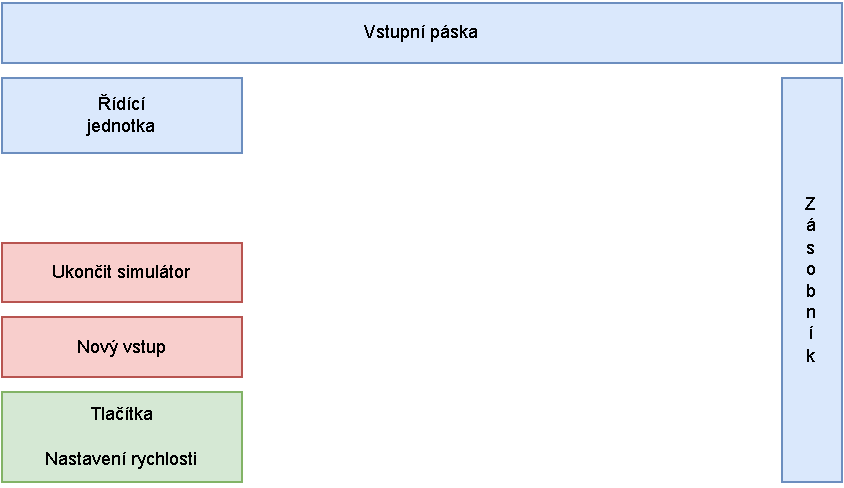
\includegraphics{Figures/SimulatoPageDesign.drawio.pdf}
    \caption{Návrh simulátoru}\label{fig:SimulatorPageDesign}
\end{figure}

Když se přesunu do kódu, jako první jsem potřeboval způsob, jak reprezentovat stav zásobníkového automatu. K tomu mi slouží PushdownAutomataSimulator. Ta obsahuje automat, na kterém probíhá simulace, vstupní pásku, zásobník, aktuální stav, přijímací stavy a historii použitých přechodových funkcí, viz obrázek~\ref{fig:SimulatorClasses}. Metoda reset slouží k zresetování simulátoru do výchozího stavu a applyTransitionFunction přijme jako parametr přechodovou funkci a upraví podle ní stav simulátoru. Následující tři metody neupravují nijak stav simulátoru, ale pouze vrací informace pomocí návratových hodnot. Metoda acceptedInput vrací hodnotu true/false podle toho, zda byl vstup přijat. Pokud není vstup celý přečtený, vrátí false. Pokud je přečtený, tak záleží na typu automatu, buď vrátí hodnotu podle toho, zda je zásobník prázdný nebo ne, nebo podle toho, zda je aktuální stav v množině přijímacích stavů.
Poslední dvě metody, nextStep a backStep, vrací přechodové funkce, které mohou být použity pro posun dopředu, respektive dozadu.

\begin{figure}[h]
    \centering
    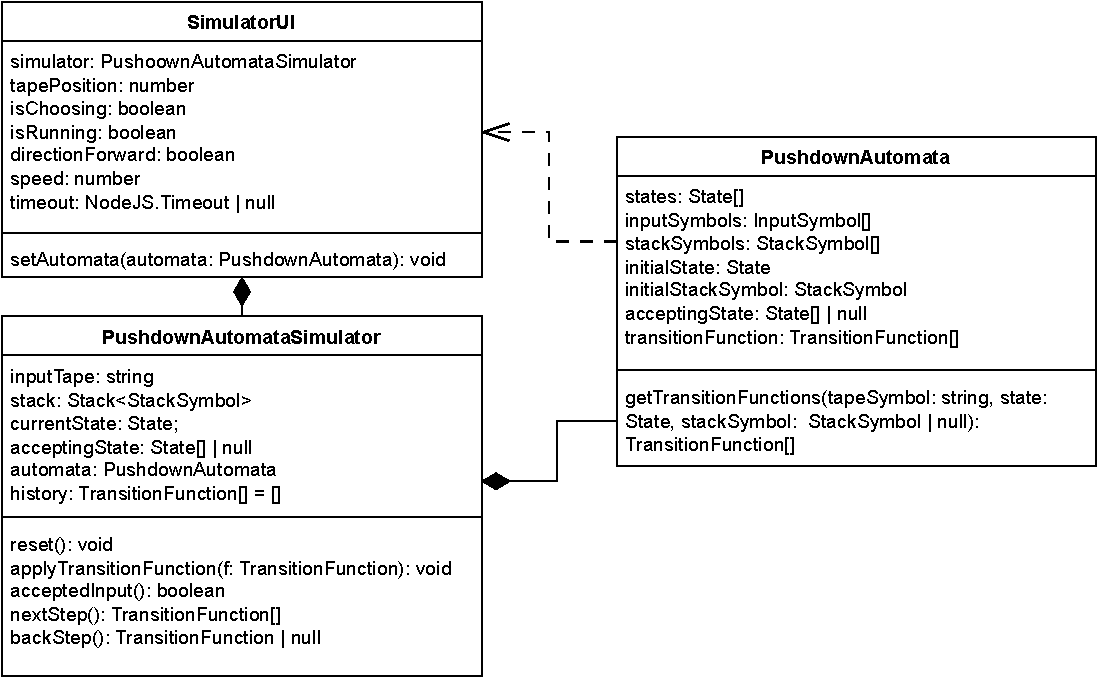
\includegraphics[width=\textwidth]{Figures/SimulatorClasses.drawio.pdf}
    \caption{Třídní diagram tříd simulátoru}\label{fig:SimulatorClasses}
\end{figure}

Nejrozsáhlejší třídou simulátoru je pak třída SimulatorUI.\ Na obrázku~\ref{fig:SimulatorClasses} jsou jen některá atributy a metody této třídy. Kromě nich dále obsahuje spoustu atributů, které si ukládají odkazy na jednotlivé části UI, a metody, pomocí kterých jde s UI manipulovat. Díky tomuto může tato třída obstarávat vše, co uživatel vidí a udělá.

Když se uživatel přepne na stránku simulátoru, jako první se zavolá metoda setAutomata. Ta nastaví simulátor s uživatelem vybraným zásobníkovým automatem a zresetuje celé UI, což obnáší vyčištění vstupní pásky, zásobníku a řídící jednotky, historie použitých přechodů a nastavení výchozích hodnot z automatu. Dále se nastaví výchozí hodnoty proměnných potřebných pro automatickou simulaci --- isChoosing, isRunning, directionForward, speed a timeout. Nakonec se otevře vyskakovací okno pro zadání slova na vstupní pásku. Toto okno obsahuje jednoduchý formulář s pouze jediným vstupem, nad kterým při každé změně proběhne kontrola, zda obsahuje pouze symboly vstupní abecedy. Když uživatel vstup potvrdí, znovu se zkontroluje, zresetuje se UI a vstup se nastaví do vstupní pásky.

K ovládání uživateli slouží 5 tlačítek a posuvník, obrázek~\ref{fig:SimulatorButtons}. Krajní tlačítka slouží k zapnutí automatické simulaci. Středové tlačítko slouží k pozastavení automatické simulace a posuvník níže slouží k nastavení času mezi jednotlivými kroky (svou hodnotu ukládá do proměnné speed). Zbylé dvě tlačítka slouží k manuálnímu krokování simulace.

\begin{figure}[h]
    \centering
    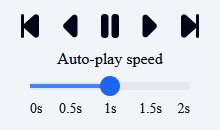
\includegraphics{Figures/PrntScrn_SimulatorButtons.png}
    \caption{Ovládací tlačítka simulátoru}\label{fig:SimulatorButtons}
\end{figure}

Pokud uživatel zmáčkne tlačítko pro krok dopředu, jako první se zkontroluje, zda aktuálně nevybírá přechodovou funkci. K tomu slouží atribut isChoosing. Pokud je aktuálně v tomto výběru a chce udělat krok v před, je na to upozorněn probliknutím oblasti s výběrem přechodových funkcí. Pokud v tomto výběru nebyl, pomocí metody nextStep třídy PushdownAutomataSimulator se zjistí všechny přechodové funkce, které je možné pro další krok použít. Podle počtu navrácených přechodových funkcí mohou nastat tři situace:
\begin{itemize}
    \item Pokud metoda nevrátila žádnou přechodovou funkci, pozastaví se automatická simulace, pokud byla zapnuta, a vyhodnotí se, zda byl vstup přijat.
    \item  Pokud metoda vrátila právě jednu přechodovou funkci, je tato funkce použita. Pokud byla zapnuta automatická simulace, což se zjistí podle proměnné isRunning, nastaví se automatické zapnutí dalšího kroku podle aktuální hodnoty atributu speed a uloží se do atributu timeout.
    \item Pokud metoda vrátila více přechodových funkcí, nastaví se atributu isChoosing na true a vygenerují se tlačítka se všemi možnostmi.
\end{itemize}

Když je použita přechodová funkce, musí se provést postupně několik věcí. Nejprve se změní vnitřní stav simulátoru metodou applyTransitionFunction. Následně se změní stav řídící jednotky. Pokud byl přečten symbol ze vstupní pásky (nebyl to epsilon přechod), spustí se funkce moveTape. Ta inkrementuje hodnotu atributu tapePosition a změní styly přilehlý symbolů --- přečtený dostane světlejší barvu a následující symbol dostane barvu tmavší. To umožní uživateli jednodušeji poznat, kterým symbol bude čtený v dalším kroku. Následně se odebere vrchní symbol ze zásobníku a přidají se symboly nové, pokud je přechodová funkce obsahuje. Následně se uloží nový záznam do historie. Nakonec se ještě zkontroluje, jestli již nebylo slovo zásobníkovým automatem přijato.

Pokud bylo možné použít více než jednu přechodovou funkci, generují se tlačítka pro jednotlivé přechodové funkce, obrázek~\ref{fig:TransitionFunctionChoosing}. Pro každé tlačítko je přidán event, který se spustí po kliknutí. Použije se konkrétní přechodová funkce a pokud byla zapnuta automatická simulace, nastaví se automatické zapnutí dalšího kroku podle aktuální hodnoty atributu speed a uloží se do atributu timeout.

Pokud uživatel zmáčkne tlačítko pro krok dozadu, jako první se zkontroluj, zda uživatel zrovna nevybírá přechodovou funkci. Pokud ano, výběr se schová. Pokud ne, získá se z historie poslední použitá přechodová funkce a náležitě se upraví stav simulátoru. Jestliže je zapnutá automatická simulace, nastaví se automatické zapnutí předchozího kroku podle aktuální hodnoty atributu speed a uloží se do atributu timeout. Ve chvíli, kdy je historie prázdná, nachází se simulátor ve výchozím stavu a pokud je zapnutá automatická simulace, vypne se.

\begin{figure}[h]
    \centering
    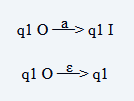
\includegraphics{Figures/PrntScrn_TransitionFunctionChoosing.png}
    \caption{Volba přechodových funkcí}\label{fig:TransitionFunctionChoosing}
\end{figure}

Na začátku kapitoly jsem zmínil, že mi mezi ovládacími prvky a zásobníkem zůstalo prázdné místo, obrázek~\ref{fig:SimulatorPageDesign}. Toto místo jsem využil pro zobrazování dvou informací. První je tabulka zobrazující definici aktuálně používaného automatu. Druhou je pak historie použitých přechodových funkcí, které se v průběhu simulace použily. V případě mobilního zobrazení stránky jsou tyto informace schovány v modálním okně, které lze otevřít tlačítkem.

\section{Úložiště}
V kapitole~\ref{sec:AppRequirements} bylo specifikováno, že si aplikace bude ukládat veškeré automaty, aby se k nim mohl uživatel kdykoliv vrátit. K tomu aplikace využívá Local Storage.\footnote{https://developer.mozilla.org/en-US/docs/Web/API/Window/localStorage}. Local storage je úložiště v prohlížeči, které umožňuje ukládat data na straně klienta. Tyto data jsou ukládaná ve formě key-value, kdy pro každý klíč existuje jedna hodnota. Na rozdíl od session storage, kdy dochází k vymazání dat po opuštění stránky, zde data zůstávají i po opuštění stránky nebo zavření prohlížeče.

V mé aplikaci jsem si pro práci s tímto úložištěm udělal třídu Storage, zkrácený zápis lze vidět ve zdrojovém kódu~\ref{src:StorageClass}. Jelikož Local Storage umožňuje ukládat klíče a hodnoty pouze jako textové řetězce, udělal jsem si nejprve metody save, která hodnotu převede na text a uloží ji do úložiště, a load, která pro zadaný klíč načte hodnotu z úložiště a převede ji z textu zpět na zadaný datový typ nebo objekt. Pro převody používám javascriptové funkce $JSON.stringify()$ a $JSON.parse()$. Dále jsem si vytvořil metodu saveAutomata, která si nejprve ověření, zda už neexistuje v úložišti záznam se stejným klíčem pomocí funkce keyExist. Pokud existuje, zeptá se uživatele, zda tento záznam může přepsat. Následně pomocí metody save uloží automat. Metoda loadAutomata si načte pro zadaný klíč automat z úložiště funkcí load, nastaví mu správný prototype a vrátí ho návratovou hodnotou. 

\begin{lstlisting}[label=src:StorageClass, caption={třída Storage}]
    class Storage{
        save<T>(key: string, item: T);
        load<T>(key: string): T | null;
        saveAutomata(key: string, automata: PushdownAutomata): boolean;
        loadAutomata(key: string): PushdownAutomata | null;
        delete(key: string);
        keyExists(key: string): boolean;
        loadFile(e: SubmitEvent);
        insertRow(key: string);
        printAutomatas();
        showAutomata(key: string);
    }
\end{lstlisting}

Metoda printAutomatas slouží k výpisu všech automatů uložených v paměti. Metoda iteruje skrze všechny klíče v úložišti a volá pro ně metodu insertRow. Ta si pro zadaný klíč načte automat z úložiště a uloží nový řádek do tabulky i se všemi příslušnými tlačítky a nastavenými událostmi:
\begin{itemize}
    \item Zobrazení specifikace automatu --- metoda showAutomata
    \item Spuštění simulátoru
    \item Editace automatu
    \item Stažení automatu jako soubor typu JSON (JavaScript Object Notation)
    \item Odstranění automatu z úložiště --- metoda delete
\end{itemize}


Poslední důležitou je metoda loadFile sloužící k nahrání automatu ze souboru. Tato metoda je nastavená jako submit event, spustí se tedy pouze při odeslání formuláře. Formulář obsahuje pouze dvě pole. První je textové a slouží pro pojmenování automatu. Toto jméno se zobrazuje ve výpisu všech automatů a zároveň je použito jako klíč pro ukládaní. Druhé pole pak slouží pro nahrání souboru. Po odeslaní se formuláře se spustí metoda loadFile, která nejprve zkontroluje, že jsou obě pole vyplněné. Následně si pomocí metody keyExists zjistí, jestli klíč již není náhodou použit a případně se uživatele zeptá, zda chce automat pro ten klíč přepsat. Poté se ze souboru pokusí vytvořit objekt typu PushdownAutomata a provede na kontrolu, zda je automat správně nadefinován, pomocí funkce checkPushdownAutomata. Pokud se nevyskytla žádná chyba, přepne uživatele do simulátoru s nastaveným aktuálně nahraným zásobníkovým automatem.

\section{Stránka pro tvorbu zásobníkových automatů}\label{sec:PDABuilderImplementation}

Třída formAutomataBuilder slouží k obsluze stránka, který slouží k tvorbě zásobníkového automatu. Obsahuje funkce, které se starají o zpracování dat při odeslání formulářů, kontroly dat, zobrazování chybových hlášek a další. Stránka se skládá z několika částí, kdy každá část odpovídá jedné části zásobníkového automatu. 

První částí je formulář pro přidávání stavů. Po jeho odeslání se přidá nový stav do množiny stavů a přidá se jako jedna z možností, kterou lze vybrat jako přijímací stav a jako počáteční stav. Pokud je stav odstraněn, musí se odstranit i jako možnost v obou výběrech. Další částí je formulář pro přidávání symbolů vstupní abecedy. Po odeslání se symbol uloží do množiny vstupních symbolů vstupní abecedy. Po ní následuje formuláře pro přidání symbolu zásobníkové abecedy. Ten po odeslání kromě uložení symbolu ještě symbol přidá do seznamu možností počátečního zásobníkového symbolu. Všechny tyto tři formuláře zároveň přidávají tlačítka do prvku pro tvorbu přechodové funkce. 

Následující dvě části jsou seznamy pro výběr počátečního stavu a počátečního zásobníkového symbolu. Oba tyto seznamy reagují na jakoukoliv změnu díky nastavené change události a vždy si uloží vybranou možnost. Předposlední část slouží k určení, jestli automat bude slovo přijímat prázdným zásobníkem nebo množinou přijímacích stavů. To uživatel může určit pomocí zaškrtávacího pole. Pokud pole není zaškrtnuté, zobrazí se uživatel seznam stavů a uživatel si může vybrat, které stavy budou přijímací.

Poslední část stránky slouží k definování přechodů přechodové funkce. Každý přechod se skládá z 5 částí, které můžeme vidět na obrázku~\ref{fig:FilledTransition} v prvním řádku. První 4 části jsou povinné, zatímco poslední část může zůstat prázdná dle definice přechodové funkce. Při kliknutí na kteroukoliv část se na druhém řádku zobrazí všechny možnosti, které mohou být použity pro danou část. Zobrazují se zde vždy jen aktuální symboly, které byly přidány dříve, ale pro vstupní symbol je zde ještě přidán symbol $\epsilon$. Při kliknutí tlačítka Add transition se zkontroluje, že jsou první 4 části vyplněné, že přechod obsahuje pouze symboly nadefinovaných abeced a zda tento přechod již neexistuje. Pokud je vše v pořádku, tak přidá přechod do množiny přechodů přechodové funkce.

\begin{figure}[h]
    \centering
    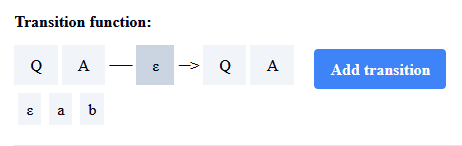
\includegraphics{Figures/PrntScrn_FilledTransition.png}
    \caption{Vyplněný přechod na stránce tvorby zásobníkového automatu}\label{fig:FilledTransition}
\end{figure}

Při kliknutí na tlačítko Save automata ve spodní části stránky se spustí funkce saveEventHandler. Ta jako první zkontroluje, že všechny abecedy mají minimálně jeden symbol a že uživatel vybral počáteční stav a počáteční zásobníkový symbol. Dále zkontroluje, zda se jedná o automat přijímající prázdným zásobníkem nebo přijímajícími stavy a zda je případně vybrán alespoň jeden. Poté ještě zkontroluje, zda je nadefinován alespoň jeden přechod přechodové funkce. Následně se provede kontrola celého zásobníkového automatu pomocí funkce checkPushdownAutomata, která je podrobněji popsána v sekci~\ref{sec:checkPushdownAutomata}. Pokud se nikde nevyskytla chyba, automat se uloží do úložiště a stránka se přepne do simulátoru.

\section{Funkce checkPushdownAutomata pro kontrolu automatu}\label{sec:checkPushdownAutomata}

Poslední důležitou částí implementace je funkce pro kontrolu definice zásobníkových automatů. Tato funkce se volá při nahrání zásobníkového automatu ze souboru nebo při jeho definici přímo na stránce. Funkce postupně prochází jednotlivé části automatu a kontroluje jejich správnost. V případě nalezené chyby si uloží chybovou hlášku a na je všechny vypíše uživateli.

Jako první postupně zkontroluje množinu stavů, vstupní a zásobníkovou abecedu. U všech tří kontroluje, jestli množiny nejsou prázdné a zda neobsahují duplicity. Jelikož typescript neobsahuje datový typ char, ale pouze string, tak u abeced ještě zkontroluje, že všechny symboly jsou délky jednoho znaku.

Dále se kontroluje počáteční stav a počáteční zásobníkový symbol. U obou se zkontroluje, zda jsou součástí konkrétních množin. Pokud automat přijímá množinou přijímacích stavů, tak se pro každý přijímací stav taktéž zkontroluje, zda je součástí množiny stavů. 

Nakonec se kontrolují přechody přechodové funkce. Pro každý přechod se zkontroluje, zda všechny jeho části (oba stavy, zásobníkové symboly a symbol vstupní abecedy, pokud není $\epsilon$) jsou součástí konkrétních množin.

Nakonec se zkontroluje, jestli pole chybových hlášek je prázdné. Pokud není, tak se pomocí funkce alert zobrazí všechny chybové hlášky, viz obrázek~\ref{fig:PDACheckErrors} a funkce vrátí hodnotu false. V opačném případě vrátí funkce hodnotu true.

\begin{figure}[h]
    \centering
    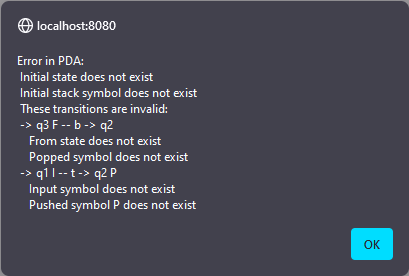
\includegraphics[width=0.6\textwidth]{Figures/PrntScrn_PDACheckErrors.png}
    \caption{Ukázka chybových hlášek kontroly zásobníkového automatu}\label{fig:PDACheckErrors}
\end{figure}

\endinput